\thispagestyle{plain}
\subsection{The Franke function}
\noindent It was stated in the project description that we should use a noise that was given by the normal distribution $\mathcal{N}(0,1)$. What we found was that since the Franke Function when plotted for $x$ and $y$ in the range between $0$ and $1$ the maximal value of the Franke function becomes around $1.4$. When plotted with noise that had values
between $0$ and $1$ the plot of the Franke function becomes unrecognizable as shown in figure \eqref{franke noise 1}. 
\begin{figure}[H]
	\centering
	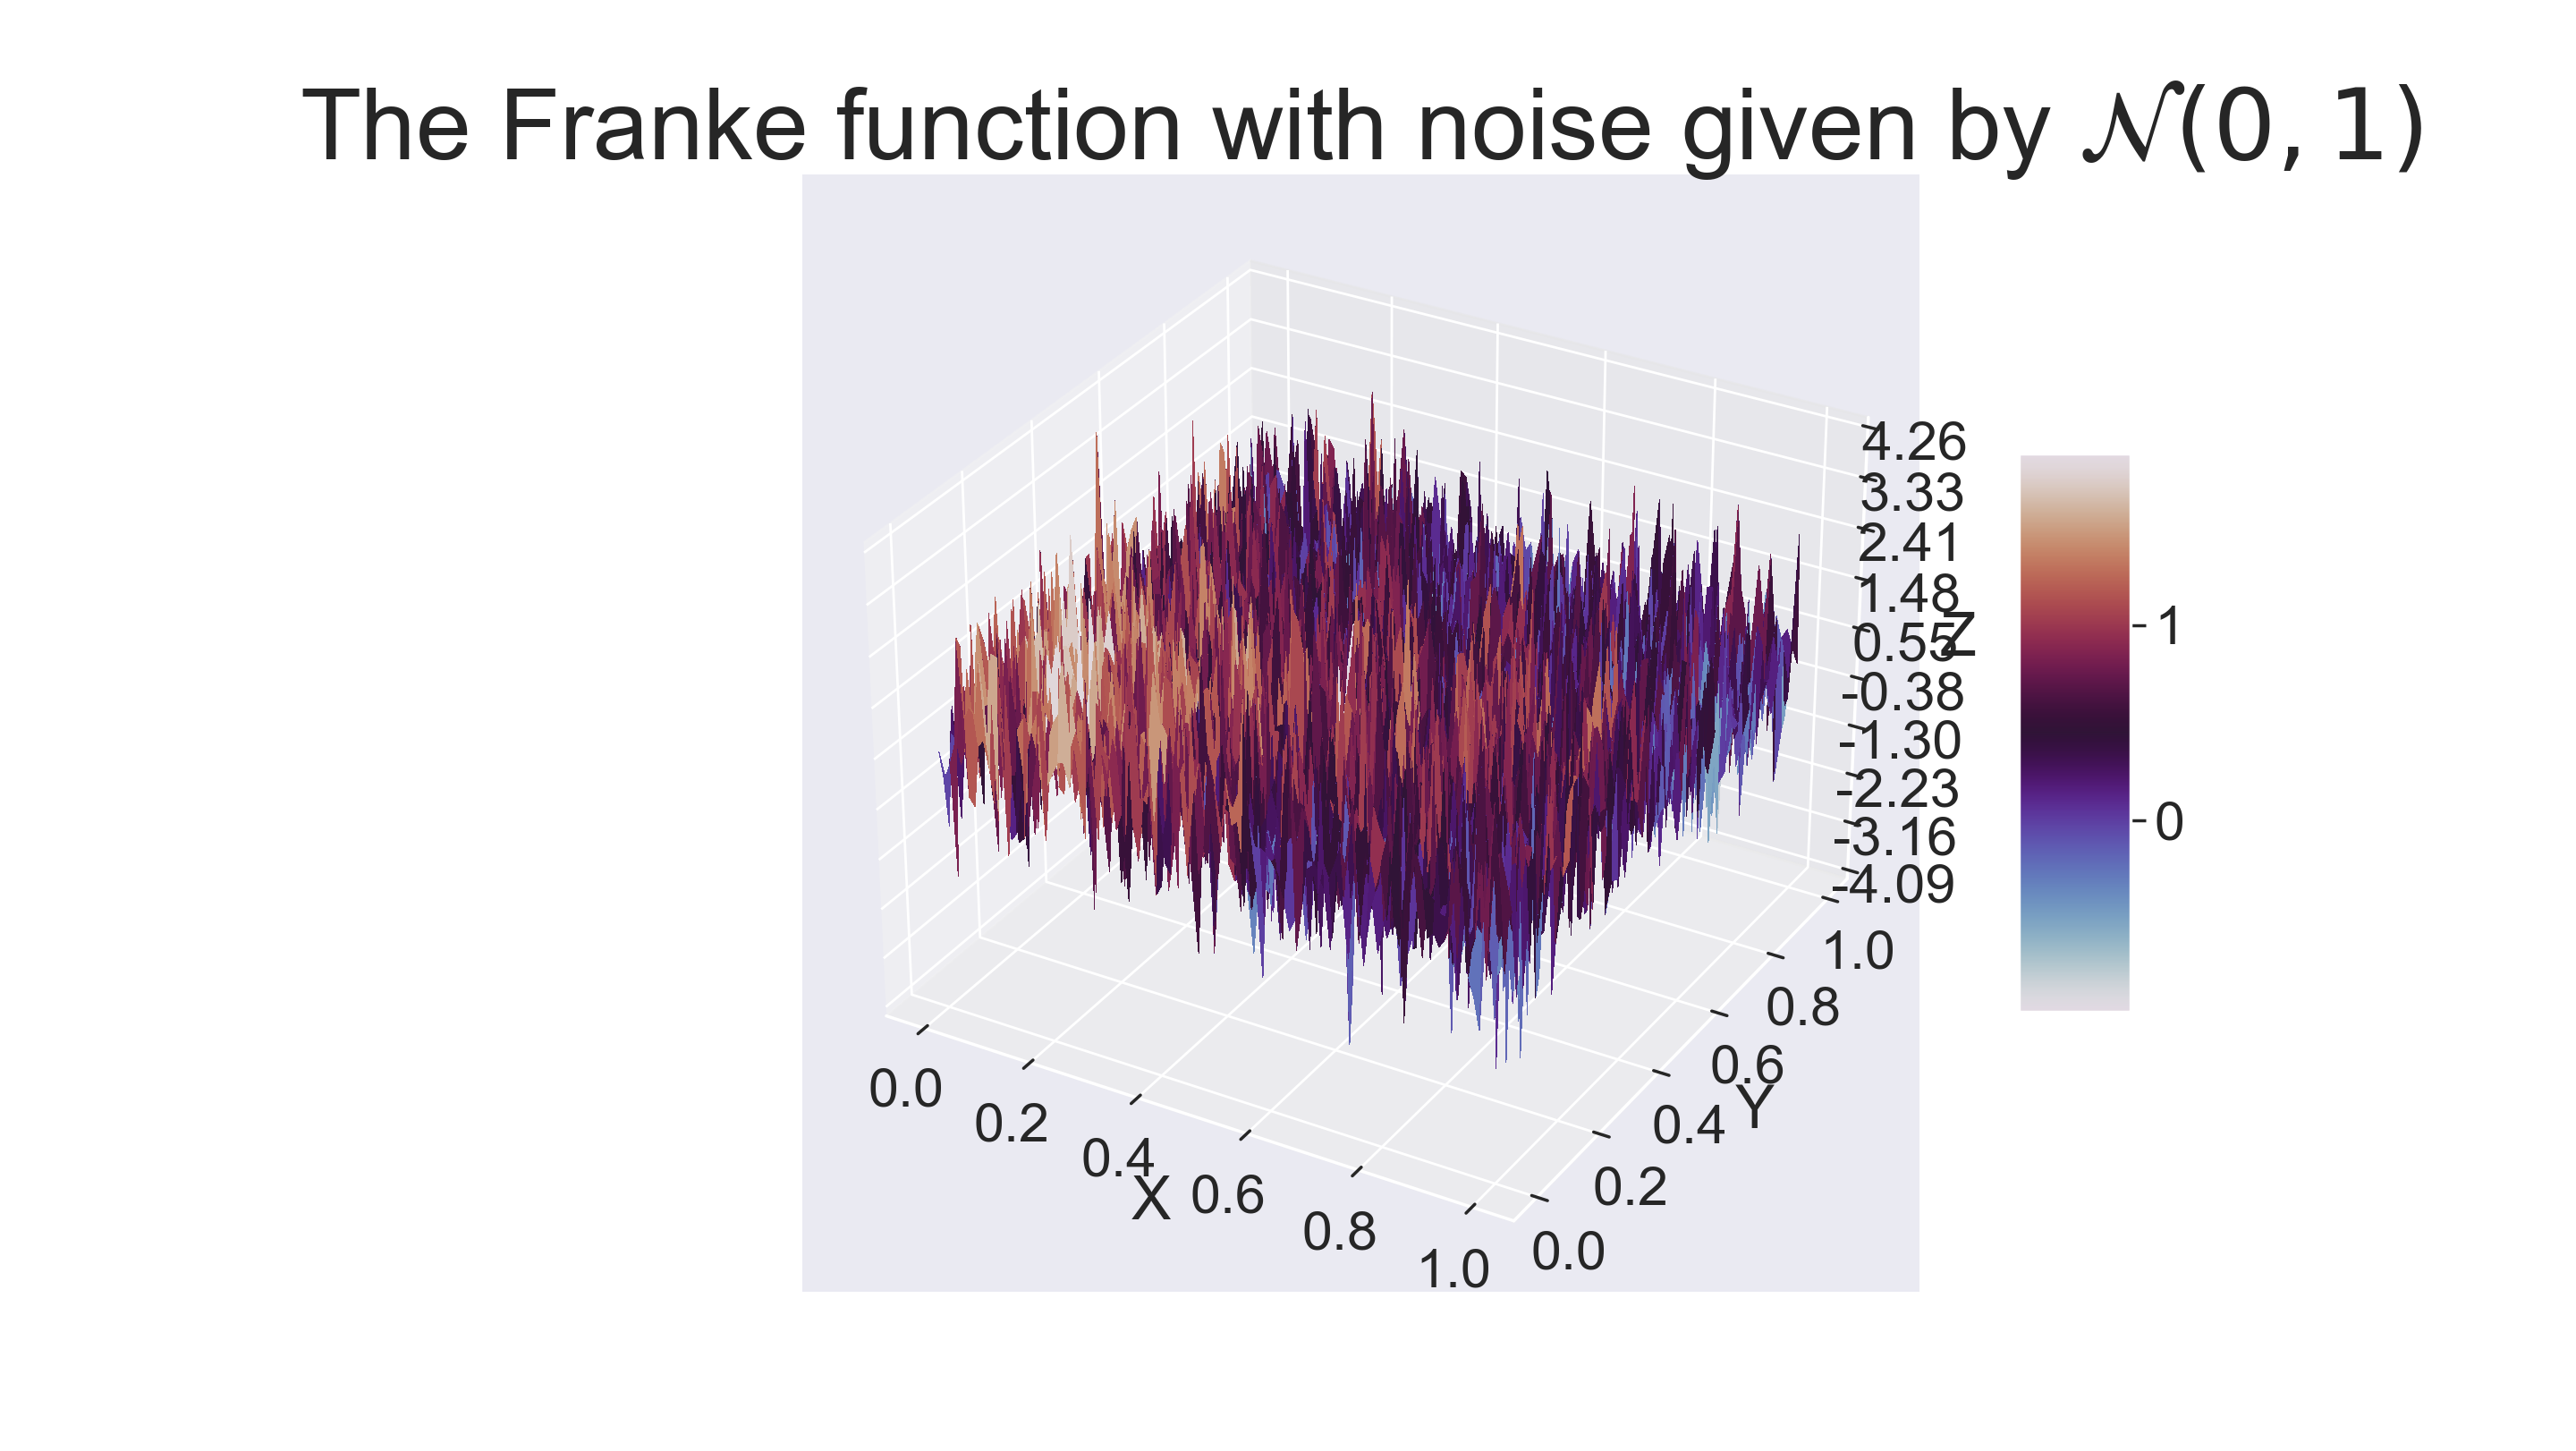
\includegraphics[width=\linewidth]{images/Figure_13.png}
	\caption{Plot showing the Franke function with noise given by the normal distribution $\mathcal{N}(0,1)$. }
	\label{franke noise 1}
\end{figure}
\noindent But if instead the normal distribution $\mathcal{N}(0,0.1)$ is 
used, the data set becomes much easier to work with, and the results becomes much prettier (as shown in figure \eqref{franke noise 0.1}) since noise has a tendency of ruining everything.
\begin{figure}[H]
	\centering
	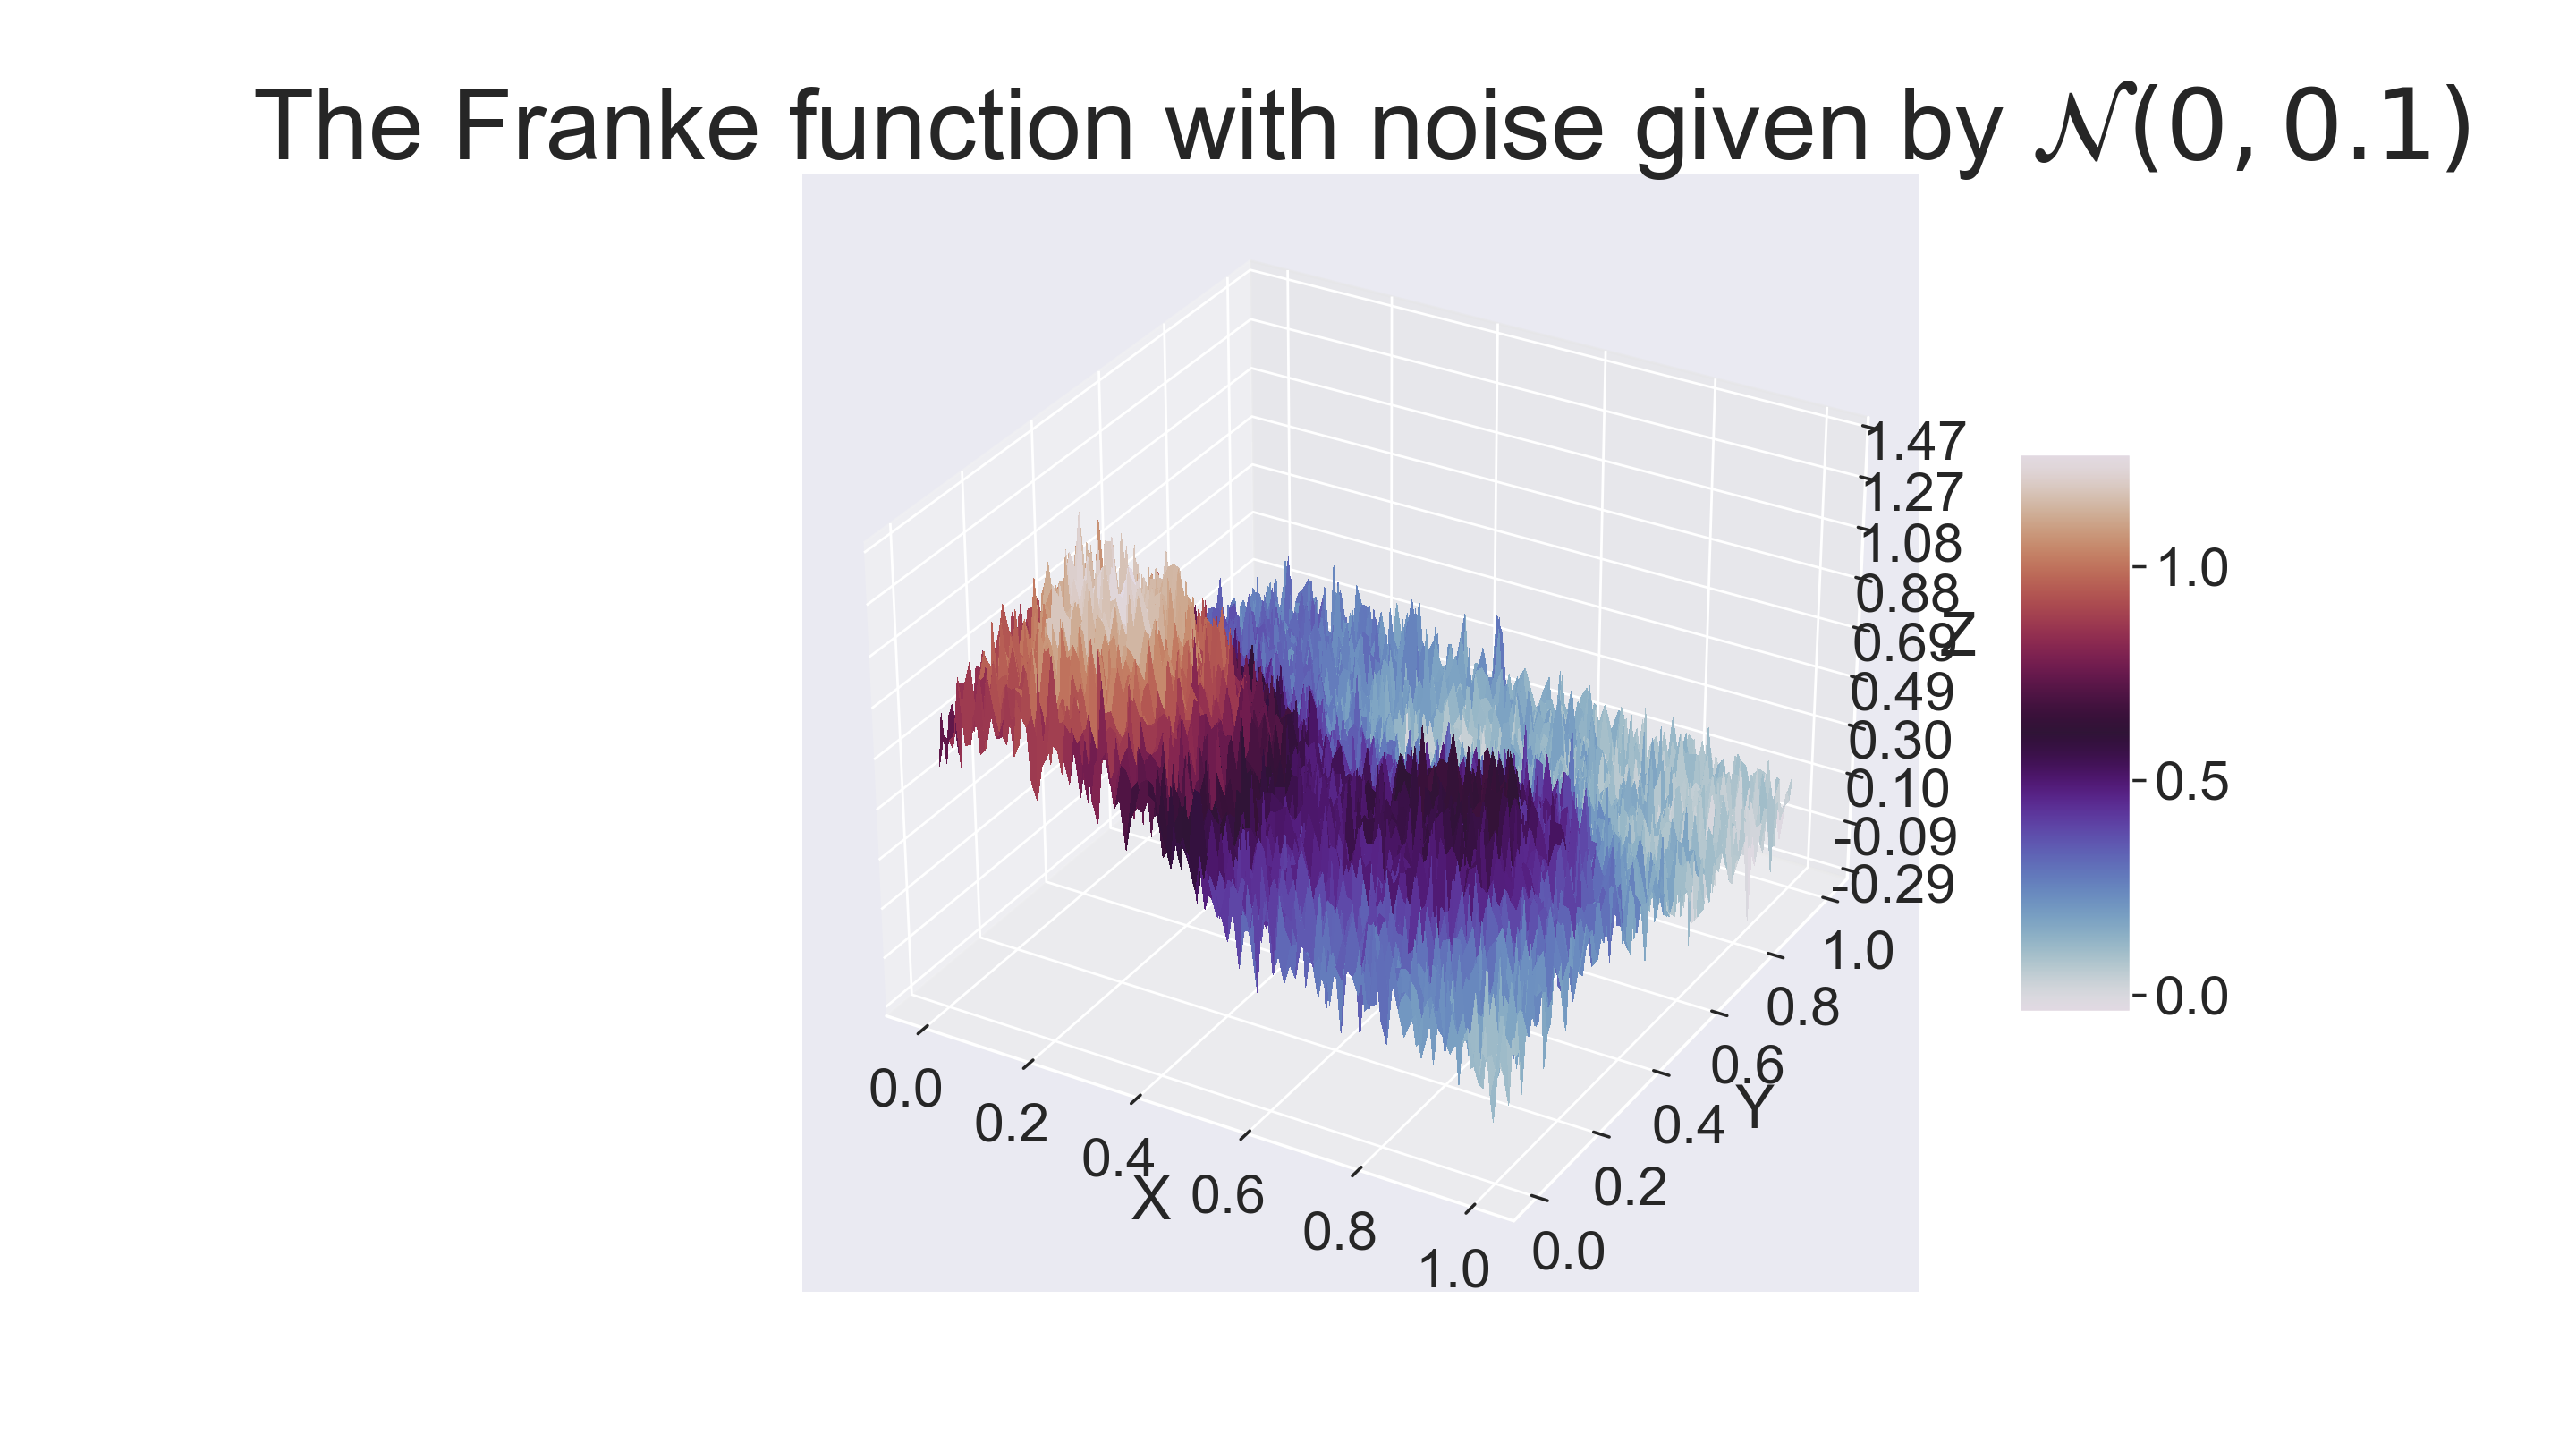
\includegraphics[width=\linewidth]{images/Figure_14.png}
	\caption{Plot showing the Franke function with noise given by the normal distribution $\mathcal{N}(0,0.1)$. }
	\label{franke noise 0.1}
\end{figure}
\noindent Now that we have gotten that out of the way, we can start actually discussing the result of the regression analysis of the Franke function.

\subsection{The Franke function}
\subsubsection{OLS}
\noindent We start with the analyses of the OLS implementation on the Franke function. It is important to note that since the parameter x and y only had values from 0 to 1 when creating the Franke function, we did not see it necessary to scale the data for any of the analysis of the Franke function, since it in a way already is scaled. The first results are the OLS model of the Franke function without noise. Figure \eqref{MSE and R2 OLS} shows the MSE and R2 scores as a function of the polynomial degree used to create the design matrix. The size of the data set analysis was a $20 \cdot 20$ matrix, were $20\%$ was put aside as test data, and the rest was used for training. What we can see from the figure is that the MSE is larger for lower polynomial degrees and starts to lower with higher values. At a fifth order polynomial degree the MSE approaches zero both for the test and training set. This is as expected, since there is no noise present there will not be any possibility for overfitting the model to the noise. Therefore the MSE will become lower and lower for higher order polynomials as shown in figure \eqref{MSE and R2 OLS}. When it comes to the R2 score we see that it becomes closer and closer to one with higher order polynomials. This is due to our model becoming increasingly better with higher orders as shown form the MSE values.

\noindent Next we look at what happens when we introduce noise given by the normal distribution $\mathcal{N}(0,0.1)$. Figure \eqref{MSE and R2 OLS noise} show the MSE and the R2 score for this case. Here we can see a classical example of overfitting the model to the noise. We see that the MSE becomes better and better for the training set but for the test set we see a sudden increase after fitting with a fourth order polynomial. This is due to the amount of data points in the different data sets, since the test data set only have $20\%$ of the original data while the training set consist of the remaining $80\%$. If we increase the number of data points the predicted model for the test data will converge towards that of the training model. 
\noindent From figure \eqref{MSE and R2 OLS} we see that when our data set does not include noise the MSE for the training data gets lower with increase in complexity, while the R2 score gets closer and closer to 1. But when we introduce noise we see from figure \eqref{MSE and R2 OLS noise} that for our test data the MSE actually increase with higher complexity. 

\noindent Next we can look at the $\beta$ values for the OLS models. What we can see from figure \eqref{beta OLS} is that for the higher order polynomials the values for the coefficients varies a lot in value. This is due to the regression method trying to fit the function to the noise, so this is a direct effect of overfitting the function with a to high order polynomial. From figure \eqref{beta OLS} we see that the beta values start to vary at as low as a fourth order polynomial and that for a fifth order polynomial the variance start to become substantially large. This is also supported by the MSE plot shown in figure \eqref{MSE and R2 OLS noise}, where we can
see that the MSE starts to gradually increase after the third order polynomial. So we clearly start to move in to the over-fit area. 

\noindent From the bootstrap results in figure \ref{fig:bootstrap_error} we can see a decrease in MSE up to polynomial degree $7$, for both the training and test data. However, we see a increase in MSE for prediction based on test data, which indicate that the model is over-fit to the training data. When we plot bias and variance, with the test error, in figure \ref{fig:bias_variance} we can see how the error decrease when the bias decrease. In addition we see increase in error when the variance increase. A decrease in the bias of the model suggest a better fit, where we reach a level of complexity to fit the data given. We also see an increase in variance for polynomial degree $7-15$, suggesting an increase in variance when we try to explain our data with higher polynomial order than necessary.

\noindent In figure \ref{fig:bias_variance} we compare the error for the Franke function, both with and without noise, with the estimated bias and variance. What we see is that MSE of the model bias follow the error up to a polynomial degree of 3 for the model with noise, and is close in value up to degree 10. At degree 10 we can see the error is close to the variance. This is expected as the error of the model can be found by summing the bias and variance \eqref{eq:bias_variance}. At the degree where both the error and variance increase, the model has become overfitted. Meaning we are training our model using unnecessary orders of polynomial degree, resulting in predictions varying. When we compare the error with the model bias and variance for the function without noise, the relation become clearer. Here the error and variance decrease more for degrees up to 7, where the bias keep decreasing and the error and variance fluctuates, and increase from degree 12. The fluctuation in MSE for the function without noise can be due to the number of samples used being small, resulting in a small data set. However, an increase in number of data points would require higher order of model complexity to fit the data. This could be studied closer by changing seed used in generating random data points.

\noindent In figure \ref{fig:cv_kfolds} the performance of an Ordinary Least Squares (OLS) regression model across varying polynomial degrees and under different k values for k-fold cross-validation. For lower polynomial degrees (around 2 to 5), the MSE remains relatively high for all k values. This suggests that a simple linear or low-degree polynomial model may not be sufficient to capture the complexity of the data. Different k values exhibit varying performance, but they all follow a similar trend across polynomial degrees. This consistency across different k values reinforces the insights drawn about the optimal polynomial degree.

\subsubsection{Ridge}
\noindent For the Ridge regression we also have to take in to account which $\lambda$ values to use in our model. To see how this value affect out model we have plotted a heat map were the MSE is plotted as a function of both different $\lambda$ values and complexity. In figure \eqref{heatmap training ridge} we see the heat map of the MSE for the training data set. From this figure we can see that for low $\lambda$ values ($\lambda<1$) the MSE is a bit below 4 which is a better result than what we got from OLS. We also see that if we increase $\lambda$ the MSE also starts to increase to about 10 for $\lambda= 10^{2}$. If we now look at a plot of how the MSE changes as a function of complexity when $\lambda=10^{-5}$ and $\lambda = 0$, so what we do is basically compere Ridge regression done with a low $\lambda$ value and OLS. We see from figure \eqref{Ridge vs OLS} that The MSE error for models fitted with polynomial of degree $0,1,2,3$ and $4$ its the same but for a model fitted with a polynomial degree of 5 the MSE is lower for Ridge regression than for OLS. This is as we expect since the extra term in the calculation for the coefficient in Ridge will try to stop the beta values from varying a lot. We can see this is the case if we look at figure \eqref{beta Ridge} were we still see that the $\beta$ values for a fit with a fifth order polynomial still varies a lot compered to lower complexity's, but it is a fair bit lower than that of OLS regression. From this we can see that if $\lambda$ is chosen correctly the model from Ridge regression is slightly better then that of OLS.

\noindent In our analysis with Ridge regression in Figure \eqref{Ridge_crossval_mse_deg}, our primary objective was to understand the model's behavior concerning varying polynomial degrees and different regularization parameters. We employed bootstrap re-sampling and cross-validation to ensure robust model evaluation and to minimize the bias-variance trade-off.

\noindent The plot showcases the model's Mean Squared Error (MSE) as a function of polynomial degrees ranging from 1 to 15. We experimented with various $\lambda$ values to discern the impact of different regularization levels. Polynomial degree denotes model complexity. As it increases, the model becomes capable of capturing intricate data patterns, but at the risk of overfitting. Our results highlight this delicate balance. At lower degrees, irrespective of regularization, the model tends to under perform, likely underfitting the data. However, for degrees between 6 to 10, a noticeable dip in the MSE is observed for certain $\lambda$ values, suggesting an optimal complexity for this data set. These insights underscore the importance of judiciously selecting the model's complexity and regularization strength to ensure balanced and optimal performance.

\subsubsection{LASSO}
\noindent For LASSO regression, we did a similar analysis to that of ridge regression. The heat maps (Figure \eqref{heat map test LASSO} and \eqref{heat map training LASSO}) shows the Mean Squared Error (MSE) as a function of different $\lambda$ values and complexity's, illustrating how the $\lambda$ value affects our model. These heat maps demonstrate that a low $\lambda$ value ($\lambda < 0.1$) and a high complexity yield a better result than a high $\lambda$ value ($\lambda > 0.1$) and a low complexity. The optimal MSE result in the heat maps occurs for $\lambda = 10^{-8}$ and degree 4, after which it gradually worsens for higher $\lambda$ values and lower complexity's until reaching $\lambda = 10^{1}$ and degree 0. In comparison to the heat maps generated for Ridge regression, the complexity appears to have significantly bigger impact on the MSE results for LASSO regression than for Ridge regression.
\noindent If we examine the line map for MSE and $R^2$ without noise (figure \eqref{MSE_and_R2_Lasso_no_noise}), we observe that LASSO with a $\lambda$ value of $10^{-5}$ produces nearly identical results to the Ridge regression and OLS. However, if we look at figure \eqref{OLS_Ridge_and_Lasso} where we plot the OLS, Ridge and LASSO when noise is added we see that the MSE for LASSO is generally allot worse compared to the two others. 
\noindent The differences between Ridge and LASSO regressions can most likely be attributed to the limited number of iterations employed. LASSO regression runs with only a small number of iterations because of the long run time. The small amount of iterations may therefore lead to a bigger tolerance that we converge against. With more iterations added, we may have achieved a better MSE for LASSO regression. From this we can see that with noise added to he Franke function, LASSO regression performs poorly compared to Ridge regression and OLS. 

\noindent In our exploration using LASSO regression, we are looking at the relationship between the model's behavior, polynomial degrees, and varying levels of the regularization parameter as denoted in Figure \eqref{Lasso_crossval_mse_deg}. Similar to our approach with Ridge regression, we employed techniques like bootstrap re-sampling and cross-validation to provide a comprehensive evaluation and to mitigate the effects of bias and variance in our model.

\noindent The depicted plot showcases the Mean Squared Error (MSE) as a function of polynomial degrees, spanning from 1 to 15, under diverse regularization strengths ($\lambda$ values). The choice of $\lambda$ in LASSO regression is critical. It not only regularizes the model but can drive certain feature coefficients to absolute zero, effectively performing feature selection.

\noindent From our results, it's evident that for extremely low regularization strengths, specifically $\lambda =10^-8$ and $\lambda=10^-6$, the MSE remains consistently high across all polynomial degrees, implying that the model may not be sufficiently regularized and might be overfitting to the training data. As we progress to moderate regularization strengths, particularly $\lambda =10^-4$ and $\lambda=10^-2$, the MSE demonstrates a dip, notably around polynomial degrees 6 to 10, suggesting these might be optimal model complexities for this data set under the given regularization. The MSE for higher regularization strengths like $\lambda =10^0$ and $\lambda=10^2$ seems to flatten out, indicating that excessive regularization might be nullifying the effect of added model complexity, leading to underfitting.

\subsection{Real terrain data}
\subsubsection{OLS}
\noindent We started by implementing OLS regression on the real terrain data. Figure \eqref{OLS terrain data} shows the MSE and R2 score as a function of complexity. As we can see from this figure the MSE is low, this is due to the way we have scaled the data set, Without proper scaling, the MSE would have been considerably higher due to the way our data set looks. Due to this scaling the result for each of out regression methods will not differ that much. What we see from figure \eqref{OLS terrain data} is as expected since the MSE decreases with complexity. As Figure \eqref{OLS terrain data} illustrates, our observations align with expectations: the MSE tends to decrease as model complexity increases. Notably, for a polynomial fit with a degree of 10, the MSE approaches zero, suggesting that a polynomial of this degree provides a accurate approximation of the true terrain data. This is again validated by looking at the R2 score, we see that when the complexity increases the R2 score begins to converge toward a value of one, which is expected when the MSE start to get closer and closer to zero. In the case with the terrain data we will continuously see that the results for our training and testing sets are almost identical, this is due to our data set being much larger than that of the Franke function, so the size although still being $20\%$ of the original data set, it includes a substantial number of data points, causing the model's performance to closely resemble that of the training set. 

For the comparison with cross validation and bootstrap we can see in Figure \eqref{fig:bootstrap_cv_terrain} that using cross validation as a re-sampling method we get a lower MSE. At lower polynomial degrees (around 2 to 4), both methods perform similarly with minimal MSE. However, as the polynomial degree increases to around 6, the MSE for bootstrap begins to rise sharply, indicating potential overfitting. In contrast, CV's MSE remains relatively stable until around degree 10, where it also exhibits a significant increase. This suggests that CV might be more robust against overfitting for intermediate polynomial degrees. At very high degrees (12-14), both methods show a pronounced spike in MSE, highlighting the dangers of over-complicating the model.

\subsubsection{Ridge}
\noindent The next part of the project was to implement Ridge regression on the terrain data. Here we started by plotting a heat map for both the training and testing data set as shown in figure \eqref{heat map Ridge Terrain data} and \eqref{heat map Ridge Terrain data test} Here we see as expected that lower $\lambda$ values and higher complexity's give a better MSE values than for lower complexity's and higher $\lambda$ values. We can also look at how the MSE and R2 score changes as a function of complexity for a $\lambda$ value equal to $10^{-5}$ as shown in figure \eqref{MSE Ridge terrain data}. Here we see a almost identical result as for OLS this has to do with the low $\lambda$ value that approaches zero. This can also indicate that there is no noise too overfit the model with in the data set since we saw from the Franke function that when no noise was present the OLS regression gave the best result but for polynomials with higher orders the model tried fitting to the noise, which may indicate that there is no substantial amount of noise present in the data set after scaling. We can further validate this by looking at the LASSO implementation. 

\noindent The Figure \eqref{fig:cv_ridge_terrain} illustrates the performance of Ridge Regression on real terrain data, evaluated using cross-validation, as a function of various polynomial degrees and regularization parameters ($\lambda$). At the lower end of the polynomial degree spectrum (around 0 to 2), the Mean Squared Error (MSE) is quite pronounced, hinting that simpler models might not adeptly represent the nuances of the terrain data.
There is a reduction in MSE as we move towards polynomial degrees of 4 to 6. This zone seems to offer a more accurate representation of the data without excessive complexity. The region around polynomial degrees of 4 to 6 combined with $\lambda$ values ranging from $10^{-5}$ to $10^{-3}$ appears to deliver the lowest MSE, marking it as a potential optimal setting for this data set.

\subsubsection{LASSO}
\noindent We then implemented the LASSO regression on the terrain data. Here we also plotted heat maps for both the training and test data shown in figure \eqref{Heat map LASSO terrain training} and \eqref{Heat map LASSO terrain testing}. The heat maps gave approximately the same results for the terrain data as for the Franke function. They demonstrate that lower $\lambda$ values and higher complexity's gives the best MSE values as expected. 

\noindent If we then examine the line map for MSE and $R^2$ score changes as a function of complexity for a $\lambda$ value equal to $10^{-5}$ shown in figure \eqref{MSE LASSO terrain data}, we see it is nearly identical to the results from the Ridge regression and OLS results. Based on the results for LASSO on the Franke function it may indicate that the similarity's between the results stem from there being little to no noise present in the terrain data set after scaling. 

\noindent If we look at figure \eqref{MSE for OLS, Ridge and LASSO} where we plot the OLS, Ridge and LASSO for the terrain data, we see that all the three methods gets better with higher complicity's, but LASSO is generally allot worse compared to the two others. The LASSO regression for the real data may also be worse because of she small amount of iterations that may lead to a bigger tolerance that we converge against.

\noindent The Figure \eqref{fig:cv_lasso_terrain} define the performance of LASSO Regression on real terrain data, evaluated with cross-validation, based on various polynomial degrees and regularization parameters ($\lambda$). At the initial polynomial degrees (around 0 to 2), the Mean Squared Error (MSE) is relatively high. This suggests that models of low complexity may not adequately encapsulate the intricacies present in the terrain data. The optimal region, in terms of minimizing MSE, appears to be around polynomial degrees of 4 to 6, paired with $\lambda$ values between $10^{-5}$ and $10^{-3}$. This suggests that within these parameter settings, the model performs best for the given data set.
